% Generated by thesis/ch7/exp2/networks.py -- do not edit by hand.
\begin{sidewaysfigure}
  \centering
  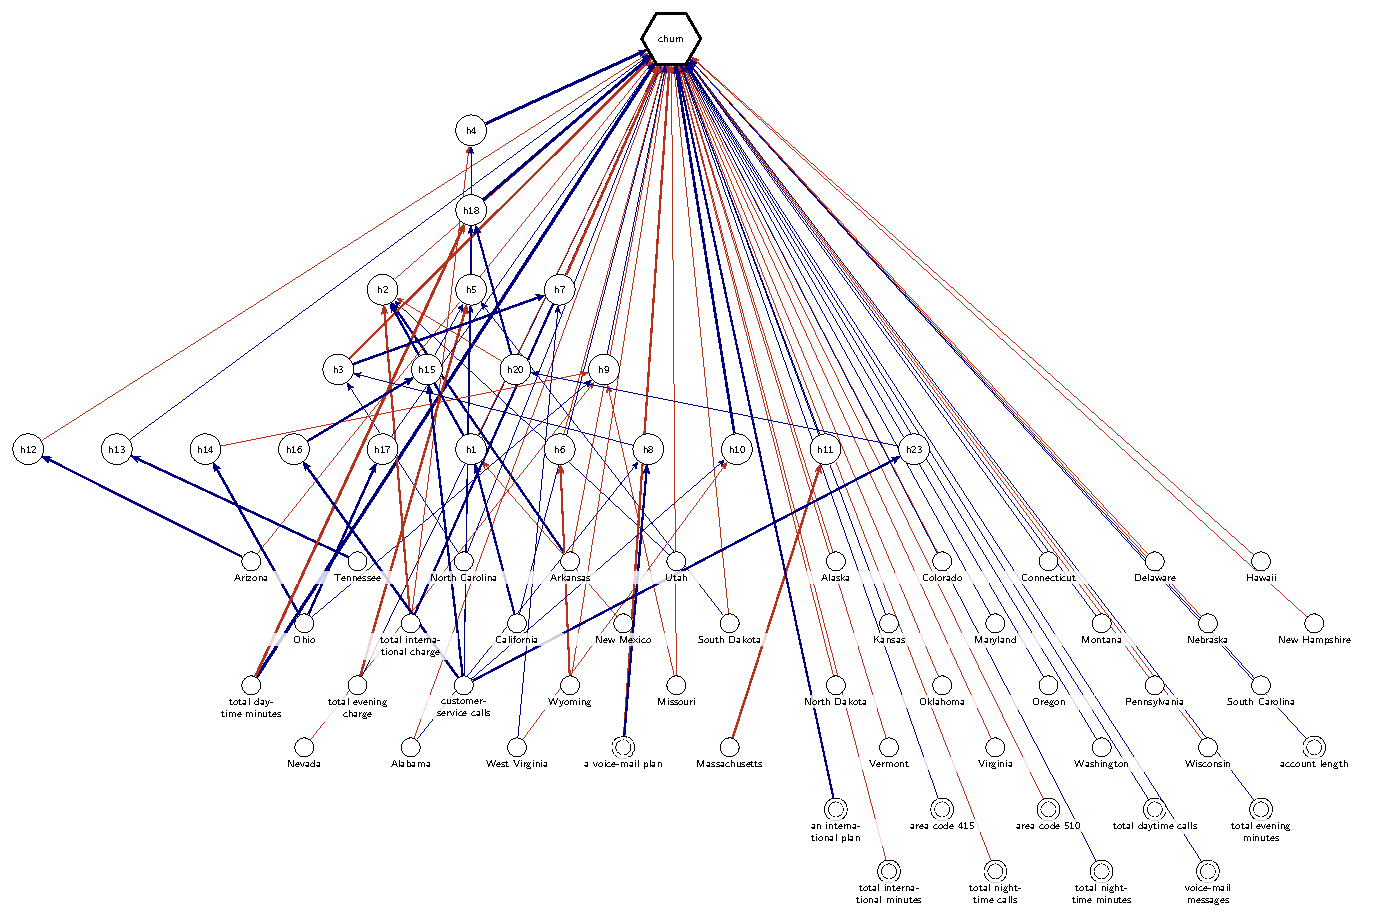
\includegraphics[width=\textheight,height=0.78\textwidth,keepaspectratio]{figures/exp2/networks/churn100-s2-raw}
  \caption{Churn, seed 2 (churn100-s2): the network as trained, before any explanation, in full. Inputs at the bottom (every input column its own node), hidden units by depth, the output at the top; 49 of 71 input columns are connected, with 20 hidden units and 94 enabled connections. Blue: positive weight (raises the score); red: negative weight (lowers it); thicker: larger weight. Orange outline and up arrow: raises the final prediction; teal and down arrow: lowers it; grey and double arrow: depends. Not used (no connection; 22 columns): Georgia, Iowa, Idaho, Illinois, Indiana, Kentucky, Louisiana, Maine, Michigan, Minnesota, Mississippi, New Jersey, New York, Rhode Island, Texas, Washington DC, Florida, area code 408, total daytime charge, total evening calls, total night-time charge and total international calls.}
  \label{fig:exp2-net-churn100-s2-raw}
\end{sidewaysfigure}
